\documentclass[11pt,a4paper]{article}

\usepackage[margin=2.5cm]{geometry}
\usepackage[T1]{fontenc}
\usepackage[utf8]{inputenc}
\usepackage{lmodern}
\usepackage{graphicx}
\usepackage{caption}
\usepackage{booktabs}
\usepackage{microtype}
\usepackage[compact]{titlesec}
\titlespacing{\section}{0pt}{0.8em}{0.3em}
\usepackage[round,authoryear]{natbib}
\usepackage[colorlinks=true,linkcolor=RoyalBlue,citecolor=RoyalBlue,urlcolor=RoyalBlue]{hyperref}
\usepackage[dvipsnames]{xcolor}

\captionsetup{font=small,labelfont=bf}
\setlength{\parskip}{0.28em}
\setlength{\parindent}{0pt}

% Every number below comes from results/summary.json, written by scripts/09_summary.py.
% Generated by scripts/09_summary.py. Do not edit by hand.
% Every number in report.tex comes from here, and therefore from results/.
\newcommand{\numDatasetDandiset}{000718}
\newcommand{\numDatasetMice}{2}
\newcommand{\numDatasetStrongShockMouse}{Ca-EEG2-1}
\newcommand{\numDatasetWeakShockMouse}{Ca-EEG3-4}
\newcommand{\numDatasetShockMaStrong}{1.5}
\newcommand{\numDatasetShockMaWeak}{0.25}
\newcommand{\numMatchingCellsTrackedStrong}{166}
\newcommand{\numMatchingCellsTrackedWeak}{223}
\newcommand{\numMatchingCellregConsensusCells}{85}
\newcommand{\numMatchingRecallMin}{0.985}
\newcommand{\numMatchingRecallMax}{1}
\newcommand{\numMatchingAgreementMin}{0.992}
\newcommand{\numMatchingAgreementMax}{1}
\newcommand{\numMatchingRecallMinPercent}{98.5}
\newcommand{\numMatchingRecallMaxPercent}{100}
\newcommand{\numMatchingAgreementMinPercent}{99.2}
\newcommand{\numMatchingAgreementMaxPercent}{100}
\newcommand{\numOverlapEnsemblePercent}{25}
\newcommand{\numOverlapRatioMin}{1.351}
\newcommand{\numOverlapRatioMax}{2.276}
\newcommand{\numOverlapSameContextFiveDaysSubject}{Ca-EEG3-4}
\newcommand{\numOverlapSameContextFiveDaysSessionA}{NeutralExposure}
\newcommand{\numOverlapSameContextFiveDaysSessionB}{Recall3}
\newcommand{\numOverlapSameContextFiveDaysDaysApart}{5}
\newcommand{\numOverlapSameContextFiveDaysSameContext}{yes}
\newcommand{\numOverlapSameContextFiveDaysActiveA}{56}
\newcommand{\numOverlapSameContextFiveDaysActiveB}{56}
\newcommand{\numOverlapSameContextFiveDaysObserved}{23}
\newcommand{\numOverlapSameContextFiveDaysExpected}{14.063}
\newcommand{\numOverlapSameContextFiveDaysRatioToChance}{1.636}
\newcommand{\numOverlapSameContextFiveDaysRatioCiLow}{1.219}
\newcommand{\numOverlapSameContextFiveDaysRatioCiHigh}{2.107}
\newcommand{\numOverlapSameContextFiveDaysJaccard}{0.258}
\newcommand{\numOverlapSameContextFiveDaysPExact}{0.002}
\newcommand{\numOverlapSameContextFiveDaysPShuffle}{0.001}
\newcommand{\numOverlapNovelContextFourDaysSubject}{Ca-EEG3-4}
\newcommand{\numOverlapNovelContextFourDaysSessionA}{NeutralExposure}
\newcommand{\numOverlapNovelContextFourDaysSessionB}{Recall2}
\newcommand{\numOverlapNovelContextFourDaysDaysApart}{4}
\newcommand{\numOverlapNovelContextFourDaysSameContext}{no}
\newcommand{\numOverlapNovelContextFourDaysActiveA}{56}
\newcommand{\numOverlapNovelContextFourDaysActiveB}{56}
\newcommand{\numOverlapNovelContextFourDaysObserved}{24}
\newcommand{\numOverlapNovelContextFourDaysExpected}{14.063}
\newcommand{\numOverlapNovelContextFourDaysRatioToChance}{1.707}
\newcommand{\numOverlapNovelContextFourDaysRatioCiLow}{1.295}
\newcommand{\numOverlapNovelContextFourDaysRatioCiHigh}{2.185}
\newcommand{\numOverlapNovelContextFourDaysJaccard}{0.273}
\newcommand{\numOverlapNovelContextFourDaysPExact}{0.001}
\newcommand{\numOverlapNovelContextFourDaysPShuffle}{0}
\newcommand{\numSimilarityDriftSpearman}{-0.817}
\newcommand{\numSimilarityDriftPShuffled}{0.006}
\newcommand{\numSimilarityDriftPairs}{10}
\newcommand{\numSimilarityDriftShuffles}{10000}
\newcommand{\numSimilarityShuffledBand}{0.148}
\newcommand{\numSimilarityPearsonMin}{0.23}
\newcommand{\numSimilarityPearsonMax}{0.572}
\newcommand{\numSimilaritySameContextFiveDaysCells}{223}
\newcommand{\numSimilaritySameContextFiveDaysPearson}{0.304}
\newcommand{\numSimilaritySameContextFiveDaysSpearman}{0.364}
\newcommand{\numSimilaritySameContextFiveDaysBinSimilarity}{0.023}
\newcommand{\numSimilaritySameContextFiveDaysPearsonShuffled}{0}
\newcommand{\numSimilaritySameContextFiveDaysPearsonShuffledPNineFive}{0.134}
\newcommand{\numSimilaritySameContextFiveDaysBinShuffled}{-0.009}
\newcommand{\numSimilaritySameContextFiveDaysPearsonCiLow}{0.179}
\newcommand{\numSimilaritySameContextFiveDaysPearsonCiHigh}{0.428}
\newcommand{\numSimilaritySameContextFiveDaysBinCeiling}{0.071}
\newcommand{\numSimilaritySameContextFiveDaysBinShareOfCeiling}{0.329}
\newcommand{\numSimilaritySameContextFiveDaysSubject}{Ca-EEG3-4}
\newcommand{\numSimilaritySameContextFiveDaysSessionA}{NeutralExposure}
\newcommand{\numSimilaritySameContextFiveDaysSessionB}{Recall3}
\newcommand{\numSimilaritySameContextFiveDaysWindow}{standard}
\newcommand{\numSimilaritySameContextFiveDaysDaysApart}{5}
\newcommand{\numSimilaritySameContextFiveDaysSameContext}{yes}
\newcommand{\numSimilarityNovelContextFourDaysCells}{223}
\newcommand{\numSimilarityNovelContextFourDaysPearson}{0.295}
\newcommand{\numSimilarityNovelContextFourDaysSpearman}{0.291}
\newcommand{\numSimilarityNovelContextFourDaysBinSimilarity}{0.036}
\newcommand{\numSimilarityNovelContextFourDaysPearsonShuffled}{-0.002}
\newcommand{\numSimilarityNovelContextFourDaysPearsonShuffledPNineFive}{0.129}
\newcommand{\numSimilarityNovelContextFourDaysBinShuffled}{-0.012}
\newcommand{\numSimilarityNovelContextFourDaysPearsonCiLow}{0.176}
\newcommand{\numSimilarityNovelContextFourDaysPearsonCiHigh}{0.405}
\newcommand{\numSimilarityNovelContextFourDaysBinCeiling}{0.067}
\newcommand{\numSimilarityNovelContextFourDaysBinShareOfCeiling}{0.54}
\newcommand{\numSimilarityNovelContextFourDaysSubject}{Ca-EEG3-4}
\newcommand{\numSimilarityNovelContextFourDaysSessionA}{NeutralExposure}
\newcommand{\numSimilarityNovelContextFourDaysSessionB}{Recall2}
\newcommand{\numSimilarityNovelContextFourDaysWindow}{standard}
\newcommand{\numSimilarityNovelContextFourDaysDaysApart}{4}
\newcommand{\numSimilarityNovelContextFourDaysSameContext}{no}
\newcommand{\numSimilarityShockContextThreeDaysCells}{223}
\newcommand{\numSimilarityShockContextThreeDaysPearson}{0.392}
\newcommand{\numSimilarityShockContextThreeDaysSpearman}{0.356}
\newcommand{\numSimilarityShockContextThreeDaysBinSimilarity}{0.056}
\newcommand{\numSimilarityShockContextThreeDaysPearsonShuffled}{-0.003}
\newcommand{\numSimilarityShockContextThreeDaysPearsonShuffledPNineFive}{0.125}
\newcommand{\numSimilarityShockContextThreeDaysBinShuffled}{-0.011}
\newcommand{\numSimilarityShockContextThreeDaysPearsonCiLow}{0.266}
\newcommand{\numSimilarityShockContextThreeDaysPearsonCiHigh}{0.511}
\newcommand{\numSimilarityShockContextThreeDaysBinCeiling}{0.08}
\newcommand{\numSimilarityShockContextThreeDaysBinShareOfCeiling}{0.701}
\newcommand{\numSimilarityShockContextThreeDaysSubject}{Ca-EEG3-4}
\newcommand{\numSimilarityShockContextThreeDaysSessionA}{NeutralExposure}
\newcommand{\numSimilarityShockContextThreeDaysSessionB}{Recall1}
\newcommand{\numSimilarityShockContextThreeDaysWindow}{standard}
\newcommand{\numSimilarityShockContextThreeDaysDaysApart}{3}
\newcommand{\numSimilarityShockContextThreeDaysSameContext}{no}
\newcommand{\numPcaVarianceFirstTwoWeak}{0.071}
\newcommand{\numPcaVarianceFirstTwoStrong}{0.136}
\newcommand{\numPcaVarianceFirstTwoWeakPercent}{7.1}
\newcommand{\numPcaVarianceFirstTwoStrongPercent}{13.6}
\newcommand{\numPcaComponentsForHalfWeak}{26}
\newcommand{\numPcaSeparationShuffledMin}{1.996}
\newcommand{\numPcaSeparationShuffledMax}{3.226}
\newcommand{\numPcaSameContextExcess}{2.286}
\newcommand{\numDecodingWithinTrainingWeak}{0.738}
\newcommand{\numDecodingWithinTrainingStrong}{0.587}
\newcommand{\numDecodingShuffledWeak}{0.498}
\newcommand{\numDecodingShuffledStrong}{0.503}
\newcommand{\numDecodingCalledShockRecallOneWeak}{0.037}
\newcommand{\numDecodingCalledShockRecallThreeWeak}{0.043}
\newcommand{\numDecodingAccuracyRecallOneWeak}{0.037}
\newcommand{\numDecodingAccuracyRecallThreeWeak}{0.957}
\newcommand{\numDecodingAccuracyRecallOneStrong}{0.52}
\newcommand{\numDecodingCalledShockRecallOneWeakPercent}{3.7}
\newcommand{\numDecodingCalledShockRecallThreeWeakPercent}{4.3}
\newcommand{\numDecodingCalledShockRecallTwoWeakPercent}{6.7}
\newcommand{\numDecodingCalledShockRecallOneStrongPercent}{52}
\newcommand{\numDecodingPooledHeldOutWeak}{0.497}
\newcommand{\numDecodingHalvesMin}{0.453}
\newcommand{\numDecodingHalvesMax}{0.573}
\newcommand{\numBehaviourFreezingStrongNeutral}{10.5}
\newcommand{\numBehaviourFreezingStrongRecallOne}{63.5}
\newcommand{\numBehaviourFreezingWeakRecallOne}{8.5}
\newcommand{\numBehaviourFreezingWeakRecallThree}{16.9}
\newcommand{\numBehaviourLargestChangeDroppingFrozen}{0.081}
\newcommand{\numBehaviourLinkSpearmanWeak}{-0.455}
\newcommand{\numBehaviourLinkPWeak}{0.187}


\title{\vspace{-1.5cm}\textbf{Drift of CA1 Context Codes Across Days}\\[0.3em]
\large Population similarity and cross-day decoding in public miniscope recordings\\
from Zaki et al.\ (2025)}
\author{Tanmay Hinge \\ \href{mailto:hingetanmay@gmail.com}{hingetanmay@gmail.com} \\
\href{https://github.com/tanmayhinge/ca1-context-drift}{github.com/tanmayhinge/ca1-context-drift}}
\date{September 2026}

\begin{document}
\maketitle
\vspace{-1em}

\section*{Abstract}

Hippocampal CA1 codes change from day to day even when the world stays the same. I asked how
much of a context remains readable in CA1 population activity days later, using the public
chronic one-photon calcium imaging of DANDI:\numDatasetDandiset{}, which holds
\numDatasetMice{} mice, up to five sessions across six days and three contexts. Cells were
followed across days with the authors' CellReg tables where those exist and with a footprint
matcher elsewhere, and the matcher recovers \numMatchingRecallMinPercent{} to
\numMatchingRecallMaxPercent{} percent of CellReg's pairs. Ensemble overlap and population
similarity exceeded chance for every session pair while failing to separate same-context pairs
from different-context pairs. Similarity fell steadily as the gap between two sessions grew
(Spearman $\numSimilarityDriftSpearman{}$, $p=\numSimilarityDriftPShuffled{}$ by shuffling,
\numSimilarityDriftPairs{} pairs). A decoder trained on day 1 against day 3 scored
\numDecodingPooledHeldOutWeak{} on held-out days, at chance.

\section{A six-day, three-context recording in two mice}

A mouse returning to a familiar room recognises it, yet the CA1 cells representing that room
partly turn over between visits, a phenomenon called representational drift
\citep{ziv2013,rule2019}. How much of a context code is still readable days later? I used the
public dataset of \citet{zaki2025}, in which mice explored a neutral context on day 1, received
three foot shocks in a different context on day 3, and returned on days 4, 5 and 6 to the shock
context, a novel context and the neutral context. CA1 was imaged with a head-mounted miniscope,
segmented with Minian \citep{dong2022}, and freezing scored from video with ezTrack
\citep{pennington2019}.

The public subset holds \numDatasetMice{} mice, and they are not replicates. The shock
amplitudes stored in the files are \numDatasetShockMaStrong{}\,mA for
\numDatasetStrongShockMouse{} and \numDatasetShockMaWeak{}\,mA for
\numDatasetWeakShockMouse{}, placing them in the two opposite groups of the original study, and
only \numDatasetWeakShockMouse{} has all five behavioural sessions. Results are therefore
reported per animal and never averaged. Files run to 2 to 5\,GB each because they carry the raw
movie, so they were read over HTTP with byte-range requests, caching only the processed traces,
footprints and behaviour, around 100\,MB.

\section{Following the same cells, and the measures applied to them}

\textbf{Following cells across days.} \numDatasetStrongShockMouse{} ships with CellReg tables
\citep{sheintuch2017}, while \numDatasetWeakShockMouse{}, the more informative animal, has
none. I aligned each session's reference image to day 1 by phase correlation, scored nearby cell
pairs by the intersection over union of their outlines, and took the best one-to-one assignment.
Because one mouse has both, the matcher was scored against CellReg before being trusted on the
other.

\textbf{Ensembles, similarity and PCA.} The planned fixed activity threshold was abandoned,
because Minian keeps only cells it detected and any fixed cut therefore labels 84 to 100 percent
of them active. An ensemble is instead the most active \numOverlapEnsemblePercent{} percent of
cells in a session, repeated at 10, 25 and 50 percent, with chance overlap from the
hypergeometric distribution and intervals from resampling cells. For similarity, each session
gives one activity rate per matched cell and those vectors are correlated between sessions, by
Pearson and by rank, against a baseline that shuffles which cell is which. Sessions were cut to
equal length, and the conditioning session contributes only its two minutes before the first
shock, since activity after a shock reflects the shock and says nothing about the room. PCA was
run on ten-second population vectors. Separation between two sessions is the standardised
difference between their time bins along the straight line joining their means, so larger values
put the sessions further apart. It was recomputed after shuffling session labels, because with
fewer time bins than cells a fitted direction separates any two groups.

\textbf{Decoding and behaviour.} A logistic regression on one-second bins of matched cells was
trained on neutral day 1 against conditioning day 3, with equal numbers of bins per class and
cross-validation over contiguous time blocks. Those two sessions fall on different days, so
context is confounded with day inside the training set and a high score there could reflect
either. The later sessions break that confound and carry the evidence below. Freezing and
ezTrack motion were measured over the same windows, and every similarity was recomputed after
discarding frozen frames.

\begin{figure}[!htbp]
\centering
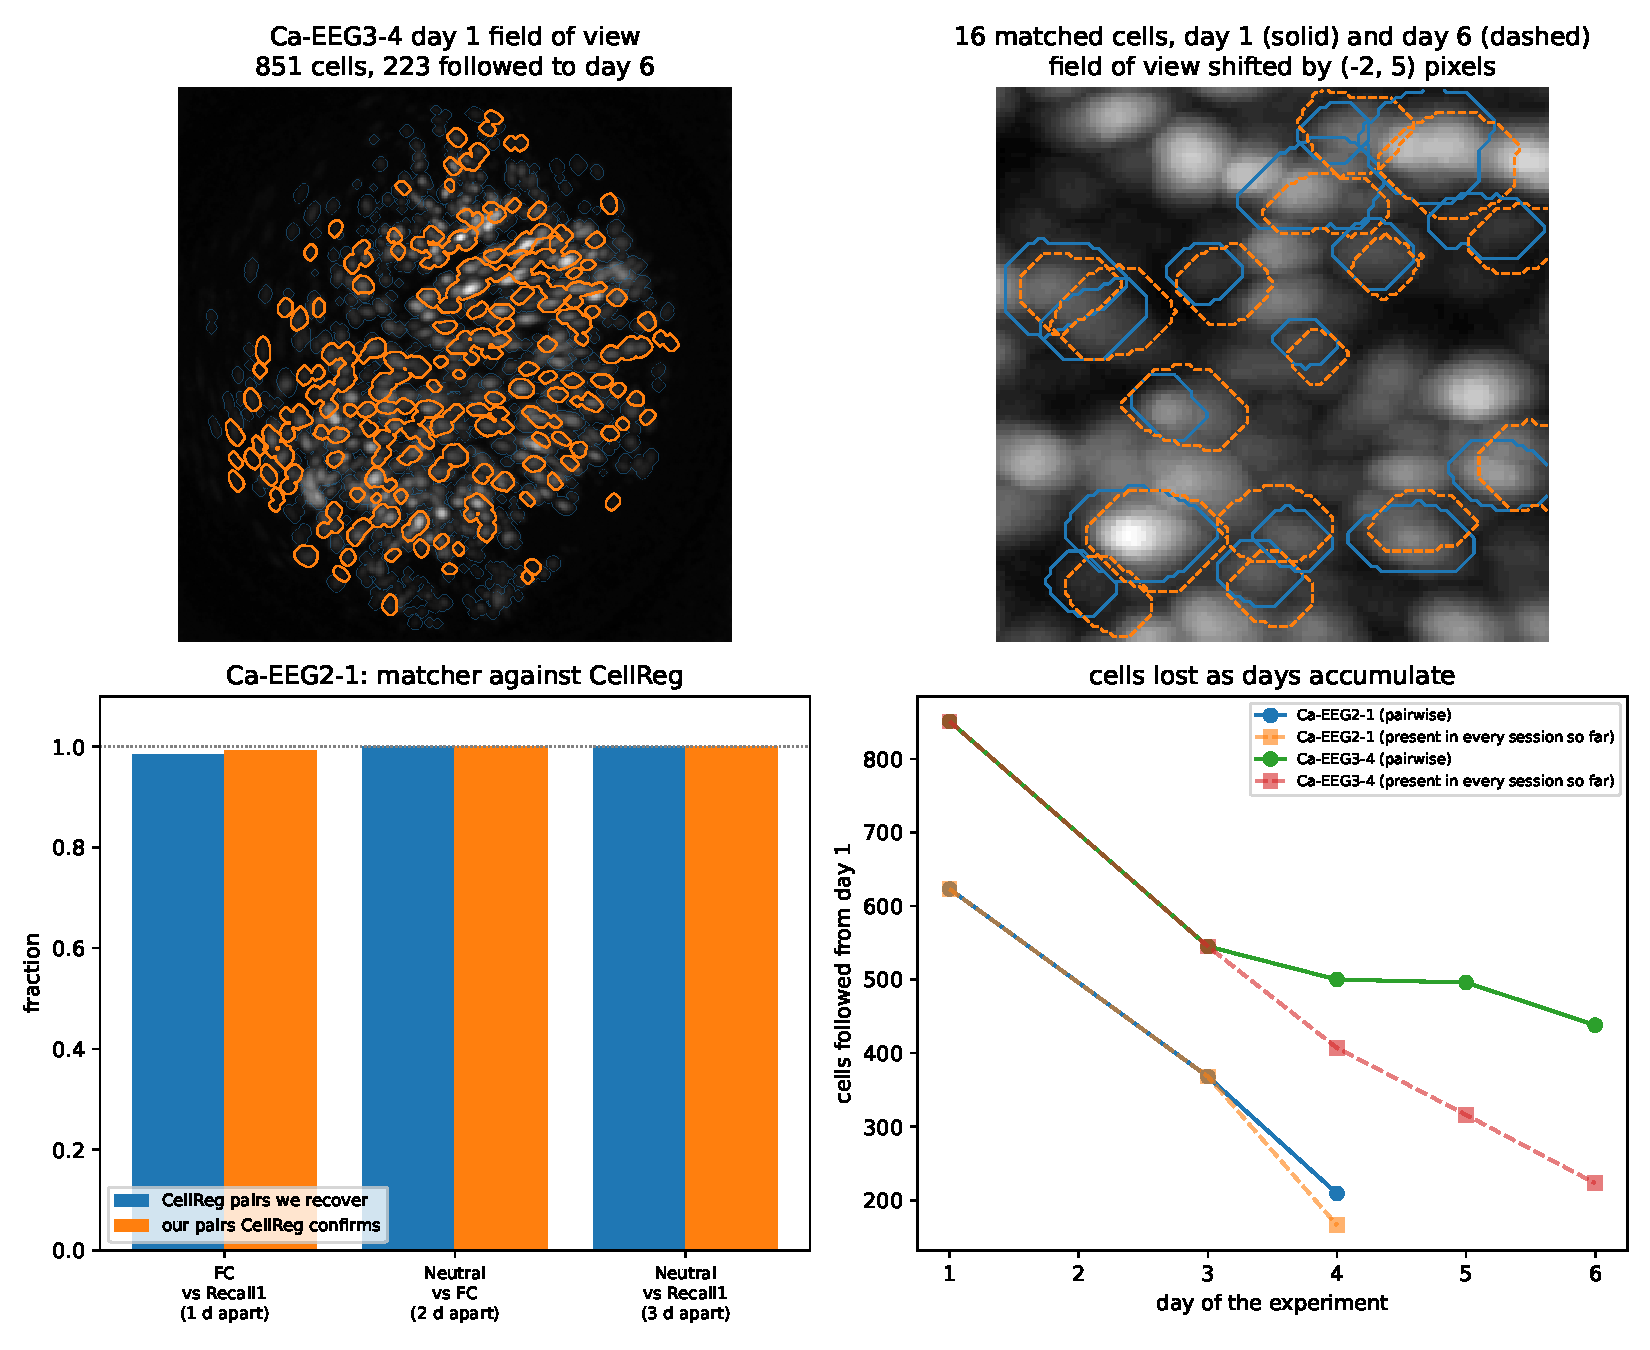
\includegraphics[width=0.92\textwidth]{../figures/02_matching.pdf}
\caption{\textbf{Cells can be followed across days, and the matcher can be checked.}
The first panel shows the day 1 field of view of \numDatasetWeakShockMouse{}, with the
\numMatchingCellsTrackedWeak{} cells followed to day 6 outlined. The second shows matched cells
on day 1 (solid) and day 6 (dashed) after aligning the two fields of view. The third reports
that on \numDatasetStrongShockMouse{}, where CellReg exists, the matcher recovers
\numMatchingRecallMinPercent{} to \numMatchingRecallMaxPercent{} percent of its pairs while
CellReg confirms \numMatchingAgreementMinPercent{} to \numMatchingAgreementMaxPercent{} percent
of ours. The fourth shows cells being lost steadily as days accumulate.}
\label{fig:matching}
\end{figure}

\section{The code drifts with elapsed time and does not identify the context}

\textbf{Cross-day matching is reliable over the gaps where it could be checked.} On
\numDatasetStrongShockMouse{} the matcher recovers \numMatchingRecallMinPercent{} to
\numMatchingRecallMaxPercent{} percent of the pairs that at least 10 of the archive's 19
independent CellReg runs agree on, and CellReg confirms \numMatchingAgreementMinPercent{} to
\numMatchingAgreementMaxPercent{} percent of ours among cells it tracked
(Figure~\ref{fig:matching}). It returns roughly twice as many pairs as that consensus. Only the
\numMatchingCellregConsensusCells{} consensus cells are independently confirmed, and the extra
pairs, which CellReg never rejected, are used here on that weaker footing. On this basis the
matcher follows \numMatchingCellsTrackedStrong{} cells across the three sessions of
\numDatasetStrongShockMouse{} and \numMatchingCellsTrackedWeak{} across all five sessions and
six days of \numDatasetWeakShockMouse{}.

\textbf{Overlap and similarity exceed chance and match across contexts.} Ensemble
overlap runs from \numOverlapRatioMin{} to \numOverlapRatioMax{} times chance, and population
correlations from \numSimilarityPearsonMin{} to \numSimilarityPearsonMax{} against a shuffled
band of $\pm\numSimilarityShuffledBand{}$ (Figure~\ref{fig:similarity}), so cross-day matching
carries real signal. The diagnostic comparison fails. For \numDatasetWeakShockMouse{},
returning to the \emph{same} neutral room after five days gives
$r=\numSimilaritySameContextFiveDaysPearson{}$ (95\% interval
\numSimilaritySameContextFiveDaysPearsonCiLow{} to
\numSimilaritySameContextFiveDaysPearsonCiHigh{}), which sits at the level of a \emph{novel}
room after four days ($\numSimilarityNovelContextFourDaysPearson{}$,
\numSimilarityNovelContextFourDaysPearsonCiLow{} to
\numSimilarityNovelContextFourDaysPearsonCiHigh{}) and below the shock room after three
($\numSimilarityShockContextThreeDaysPearson{}$). Ensemble overlap agrees, at
\numOverlapSameContextFiveDaysRatioToChance{} times chance for the same context
(\numOverlapSameContextFiveDaysRatioCiLow{} to \numOverlapSameContextFiveDaysRatioCiHigh{})
against \numOverlapNovelContextFourDaysRatioToChance{} for the novel one
(\numOverlapNovelContextFourDaysRatioCiLow{} to \numOverlapNovelContextFourDaysRatioCiHigh{}),
two intervals that overlap almost entirely.

\textbf{Elapsed time predicts similarity across all ten session pairs.} Over the
\numSimilarityDriftPairs{} session pairs of \numDatasetWeakShockMouse{}, similarity falls as
the gap between two sessions grows, with Spearman $\numSimilarityDriftSpearman{}$ and
$p=\numSimilarityDriftPShuffled{}$ from \numSimilarityDriftShuffles{} shuffles of which
similarity belongs to which gap. That correlation is the basis for reading these results as
drift in time. The PCA agrees. Its first two components hold only
\numPcaVarianceFirstTwoWeakPercent{} percent of the variance for \numDatasetWeakShockMouse{}
and \numPcaVarianceFirstTwoStrongPercent{} percent for \numDatasetStrongShockMouse{}, and
\numDatasetWeakShockMouse{} needs \numPcaComponentsForHalfWeak{} components for half of it, so
distances in such a plot are untrustworthy and the sessions overlap there. Separation along a fitted
direction is large for every pair, while shuffled session labels already give
\numPcaSeparationShuffledMin{} to \numPcaSeparationShuffledMax{}. What survives that control
orders by elapsed time, its largest excess of \numPcaSameContextExcess{} belonging to the two
visits to the \emph{same} room five days apart.

\begin{figure}[!htbp]
\centering
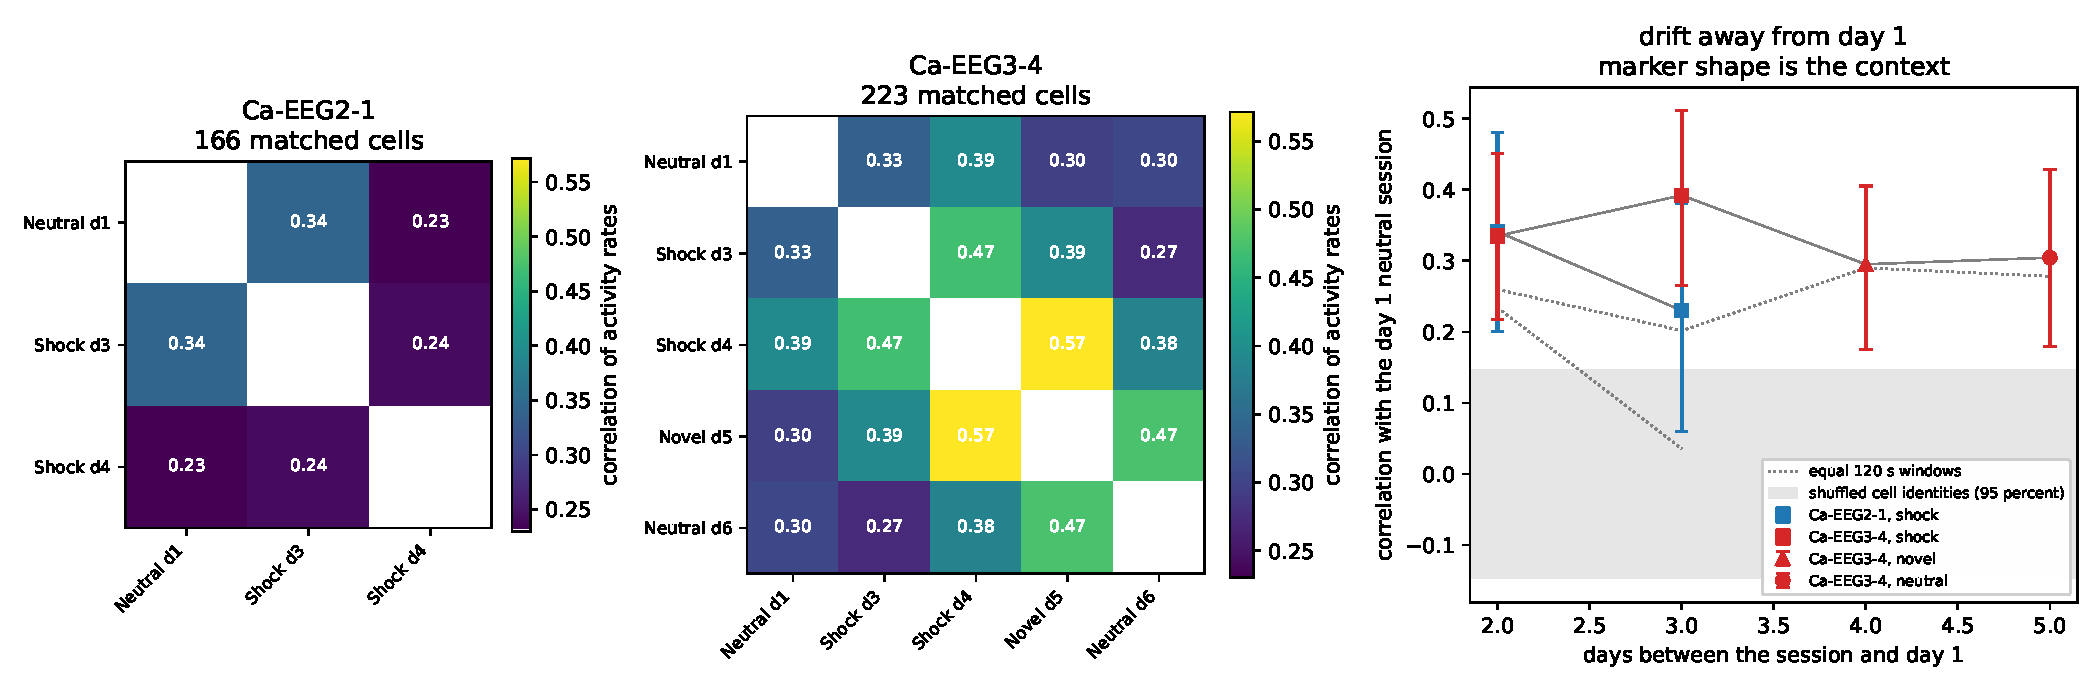
\includegraphics[width=0.92\textwidth]{../figures/04_similarity.pdf}
\caption{\textbf{Population similarity follows the calendar and ignores the context.}
Each matrix gives the correlation between per-cell activity rates for every session pair, per
animal, over matched cells. The right panel plots similarity to the day 1 neutral session
against days elapsed, with marker shape giving the context, a grey band for the shuffled
baseline and a dotted line repeating the curve with every session cut to 120\,s. The day 6
return to the neutral context sits at the level of the day 5 novel context.}
\label{fig:similarity}
\end{figure}

\begin{figure}[!htbp]
\centering
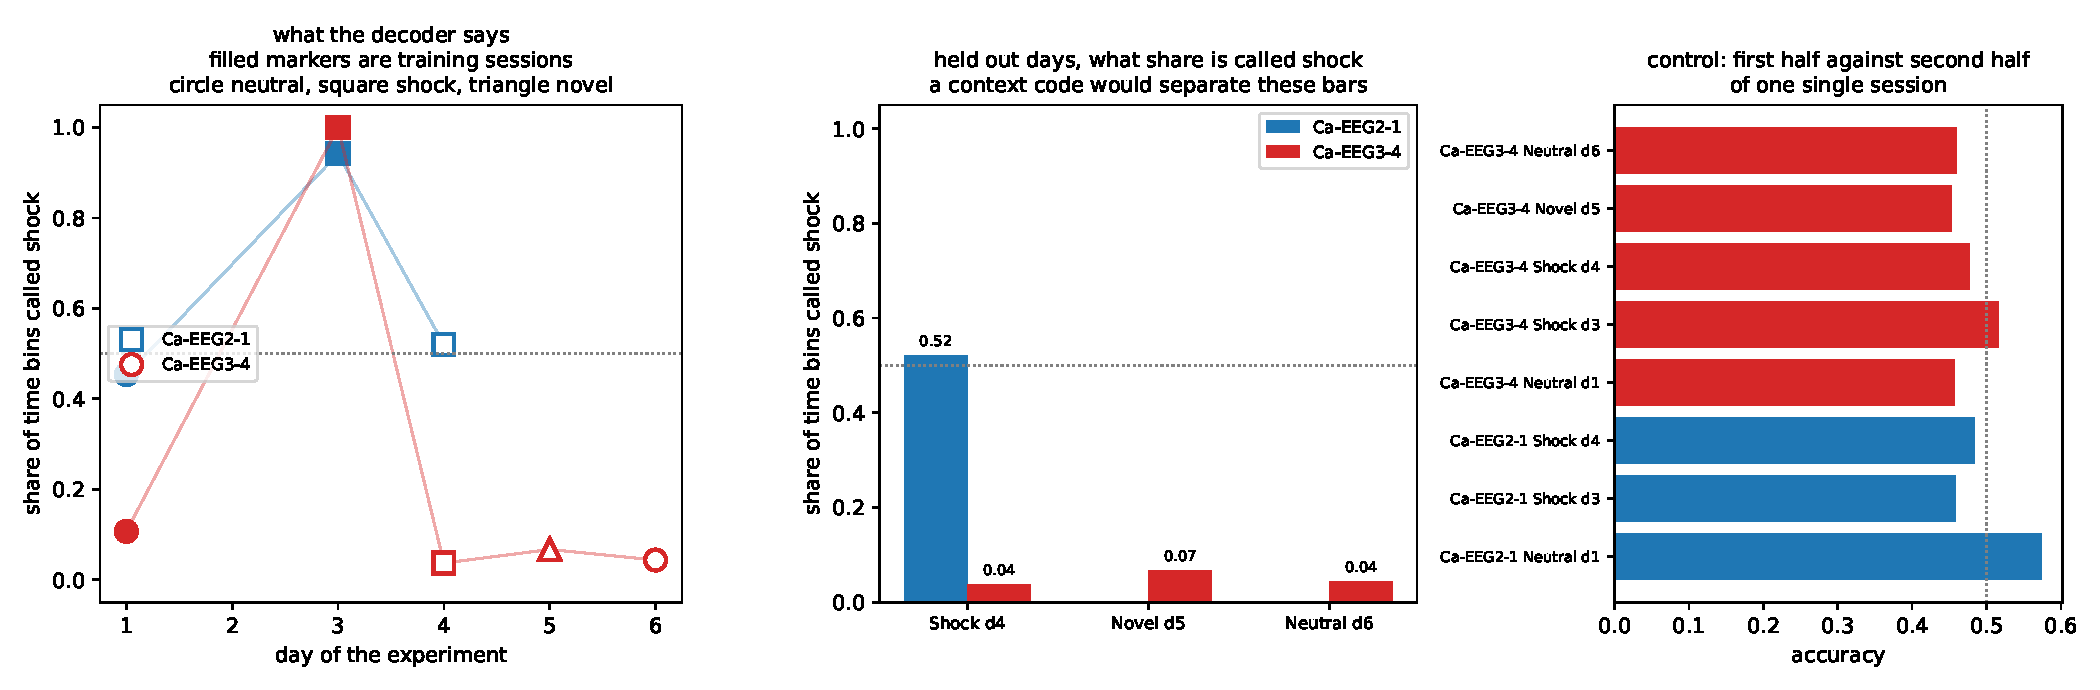
\includegraphics[width=0.92\textwidth]{../figures/06_decoding.pdf}
\caption{\textbf{A context learned on one day is not recognised on later days.} The left panel gives the
share of each session's time bins called ``shock'', with training sessions filled. The middle
panel repeats that share for the held-out days alone, where a context code would put the shock
day high and the neutral day low. The right panel is the control, telling the first half of a
single session from its second half, which sits at chance for all eight sessions.}
\label{fig:decoding}
\end{figure}

\textbf{The decoder separates the training days and stays at chance on new ones.} Within the two
training days, balanced accuracy is \numDecodingWithinTrainingWeak{} and
\numDecodingWithinTrainingStrong{} for the two mice, against an empirical chance of
\numDecodingShuffledWeak{} and \numDecodingShuffledStrong{} from shuffled labels
(Figure~\ref{fig:decoding}). Those two sessions fall on different days, so that score is
compatible with a code for the context and with a code for the day. Slow drift inside a single
recording is ruled out, since telling the first half of a session from its second half gives
\numDecodingHalvesMin{} to \numDecodingHalvesMax{} across all eight sessions. On days the decoder never saw, its answers collapse onto one
class. For \numDatasetWeakShockMouse{} it calls shock in
\numDecodingCalledShockRecallOneWeakPercent{} percent of the day 4 shock-context bins,
\numDecodingCalledShockRecallTwoWeakPercent{} percent of the day 5 novel bins and
\numDecodingCalledShockRecallThreeWeakPercent{} percent of the day 6 neutral bins, so the two
days with a correct answer pool to a balanced accuracy of \numDecodingPooledHeldOutWeak{}, at
chance. Day 4 of \numDatasetStrongShockMouse{} gives
\numDecodingCalledShockRecallOneStrongPercent{} percent, also at chance.

\textbf{Behaviour separates the two mice and leaves the neural results standing.}
\numDatasetStrongShockMouse{} froze \numBehaviourFreezingStrongRecallOne{} percent of its return
to the shock context against \numBehaviourFreezingStrongNeutral{} percent in the neutral context
on day 1, while \numDatasetWeakShockMouse{} reached \numBehaviourFreezingWeakRecallOne{} percent
there, consistent with the shock-intensity difference of \citet{zaki2025} with one animal per
condition (freezing figure in the repository). Recomputing every similarity from moving frames
only changes it by at most \numBehaviourLargestChangeDroppingFrozen{}, and behavioural and
neural change are related in the intuitive direction without being resolvable
($\rho=\numBehaviourLinkSpearmanWeak{}$, $p=\numBehaviourLinkPWeak{}$, 10 pairs).

\section{What these two mice cannot tell us}

\numDatasetMice{} mice from two shock conditions is a case study, and only one has the
three-context design, so the central negative result rests on \numMatchingCellsTrackedWeak{}
cells in a single mouse. The matcher was validated only over the
session gaps \numDatasetStrongShockMouse{} provides, which reach three days, while the
comparison carrying the argument spans five, and matching quality may fall over that longer gap.
The ten pairs behind the Spearman correlation come from five sessions and so share sessions with
one another, which is why its $p$ value comes from shuffling. Sessions run five to ten minutes with no position tracking, so a place
code could be present and invisible to session-averaged measures. The ensemble size is a choice forced by a fixed threshold labelling nearly every cell
active, and the direction of the result holds at three sizes while its magnitude does not.
Two-dimensional projections distort distances, which is why nothing rests on the PCA plot.
Failed transfer also cannot distinguish absent information from information a linear decoder on
one-second bins is unable to read.

\section{The offline recordings are the obvious next analysis}

The analysis this dataset was built for comes next, whether the neutral and shock ensembles
co-reactivate during the homecage rest recordings, already cross-registered to the encoding
sessions. Aligning activity to what the animal was doing at each moment, using all of the offline
recordings with their EEG-scored sleep states, and comparing the observed drift against a
sequence model trained on the same context sequence would each test whether elapsed time is
genuinely the organising variable.

\section{Where the code, figures and data live}

Code, figures and numbers sit at
\href{https://github.com/tanmayhinge/ca1-context-drift}{github.com/tanmayhinge/ca1-context-drift}.
Every figure regenerates from \texttt{scripts/} and every number here is read from
\texttt{results/summary.json} through generated macros, so no value is typed by hand. The data
are \href{https://dandiarchive.org/dandiset/000718}{DANDI:\numDatasetDandiset{}}
\citep{dandi000718}, used under CC-BY-4.0 and never redistributed here.

\small
\setlength{\bibsep}{3pt plus 1pt}
\bibliographystyle{plainnat}
\bibliography{references}

\end{document}
